\documentclass[UTF8,fontset=none,zihao=5,twoside,openany]{ctexbook}
\usepackage{bookstyle}
\usepackage{float}
\let\oldfigure\figure \let\endoldfigure\endfigure
\renewenvironment{figure}[1][]{\oldfigure[H]}{\endoldfigure}
\renewcommand{\cite}[1]{}
\setcounter{chapter}{4}
\pagestyle{plain}
\begin{document}

\section*{样张一：图 4-6 第二稿（按 nature-figure 示意图规范重画）}
\textbf{本稿遵守的规则：}
\begin{enumerate}
  \item 字体统一：全图一种字族、两种字号。层名用小四号加粗（全图唯一加粗处），说明与工具一律用同一号常规字体；所有文字同一深色。
  \item 结构统一：每个框内部顺序相同——层名、一行说明、底部色带写“工具：……”。工具类别因此永远出现在所属框的同一位置，不再有“向量数据库在左下、部署工具在右下”这类不一致。
  \item 尺寸统一：同一行的框等宽、等间距、上下边对齐；整幅图以正文栏中线为轴。
  \item 连线规范：连线标签与其他文字保持间距；虚线只表示一种含义（离线）。
  \item 颜色规范：唯一强调色只用于本图要表达的信息——工具类别色带；不再另用图例，色带含义写在图注里。
\end{enumerate}

\Needspace{80mm}\noindent\textbf{修改前（第一稿）}
\begin{figure}[htbp]
\centering
\begin{tikzpicture}[fig, x=1mm, y=1mm]
  \tikzset{chip/.style={draw=accent, fill=white, text=accent, rounded corners=1pt, inner sep=1.2pt,
                        font=\figfont\scriptsize, anchor=south east}}
  % 全部层宽 104 mm，以 x=0 为中心；工具类别以“标签”贴在所属层的右上角
  \node[blkw, minimum width=104mm, minimum height=9mm] (ui) at (0,0) {{\bfseries 接口层}\quad 网页 · 移动端 · 开放 API};
  \node[blka, minimum width=104mm, minimum height=11mm] (orch) at (0,-19) {{\bfseries 编排层}\\[-1pt]\footnotesize 工作流 / 智能体 · 提示词组织 · 权限校验 · 安全审查 · 日志};
  \node[blk, minimum width=36mm, minimum height=11mm] (know) at (-34,-40) {{\bfseries 知识层}\\[-1pt]\footnotesize 向量数据库 · 搜索 · 文档库};
  \node[blk, minimum width=36mm, minimum height=11mm] (model) at (6,-40) {{\bfseries 模型服务层}\\[-1pt]\footnotesize 推理引擎 · 模型 API};
  \node[blkw, dashed, minimum width=22mm, minimum height=11mm] (ft) at (41,-40) {{\bfseries 微调}\\[-1pt]\footnotesize 离线进行};
  \node[blkw, minimum width=104mm, minimum height=9mm] (infra) at (0,-59) {{\bfseries 基础设施层}\quad 计算芯片 · 存储 · 互联 · 软件栈};
  % 调用关系
  \draw[<->, line width=0.6pt] (ui.south) -- (orch.north);
  \draw[<->, line width=0.6pt] (orch.south -| know.north) -- (know.north) node[midway, right, note, font=\figfont\scriptsize] {检索资料};
  \draw[<->, line width=0.6pt] (orch.south -| model.north) -- (model.north) node[midway, right, note, font=\figfont\scriptsize] {生成回答};
  \draw[->, dashed, line width=0.6pt] (ft.west) -- (model.east) node[midway, above, note, font=\figfont\scriptsize] {权重};
  \draw[->, line width=0.6pt] (know.south) -- (know.south |- infra.north);
  \draw[->, line width=0.6pt] (model.south) -- (model.south |- infra.north);
  % 工具类别标签
  \node[chip] at ([xshift=-1.5mm]orch.north east) {编排平台 · 应用开发框架};
  \node[chip] at ([xshift=-1.5mm]know.north east) {向量数据库};
  \node[chip, anchor=north east] at ([xshift=-1.5mm]model.south east) {部署工具};
  \node[chip] at ([xshift=-1.5mm]ft.north east) {微调工具};
  \node[chip, draw=rulegray, text=rulegray] at ([xshift=-1.5mm]infra.north east) {见第 4.2 节};
  % 居中图例
  \node[chip, anchor=center] at (-20,-69) {标签};
  \node[note, anchor=west, font=\figfont\scriptsize] at (-16,-69) {五类工具各自所处的层};
\end{tikzpicture}
\caption{（修改稿）大模型应用的典型分层与五类工具的位置。编排层居中调度：检索资料和调用模型都是它发起的调用；微调在线下进行，产出的权重交给模型服务层加载}
\label{fig:s-app}
\end{figure}

\Needspace{80mm}\noindent\textbf{修改后（第二稿）}
% 图 4-6 第二稿：遵循 nature-figure 矢量示意图规范
%  - 一种字族、两种字号：层名 \small 加粗（唯一加粗处），说明与工具 \footnotesize 常规
%  - 全部文字同一深色；唯一强调色只标“工具类别”这一本图要传达的信息
%  - 同一角色的框等宽、上下边对齐；每个框内部顺序相同：层名 → 一行说明 → （底部）工具类别
%  - 连线标签与其他文字保持间距；虚线只表示一种含义：离线
\begin{figure}[htbp]
\centering
\begin{tikzpicture}[fig, x=1mm, y=1mm]
  % \layerbox{x0}{x1}{ytop}{h}{填充}{边框样式}{层名}{说明}{工具类别，可空}
  \newcommand{\layerbox}[9]{%
    \begin{scope}
      \path[clip, rounded corners=1.5pt] (#1,#3) rectangle (#2,#3-#4);
      \fill[#5] (#1,#3) rectangle (#2,#3-#4);
      \if\relax\detokenize{#9}\relax\else
        \fill[accentpale] (#1,#3-#4) rectangle (#2,#3-#4+5);
        \draw[accent, line width=0.4pt] (#1,#3-#4+5) -- (#2,#3-#4+5);
      \fi
    \end{scope}
    \draw[figline, rounded corners=1.5pt, #6] (#1,#3) rectangle (#2,#3-#4);
    \if\relax\detokenize{#9}\relax
      \node[align=center, text=ink] at ({(#1+#2)/2},{#3-#4/2})
        {{\small\bfseries #7}\\[0.5pt]{\footnotesize #8}};
    \else
      \node[align=center, text=ink] at ({(#1+#2)/2},{#3-(#4-5)/2})
        {{\small\bfseries #7}\\[0.5pt]{\footnotesize #8}};
      \node[text=ink, font=\figfont\footnotesize] at ({(#1+#2)/2},{#3-#4+2.5}) {工具：#9};
    \fi
  }
  % ---- 第 1 层 ----
  \layerbox{-55}{55}{0}{11}{figfill}{}{接口层}{网页 · 移动端 · 开放 API}{}
  % ---- 第 2 层 ----
  \layerbox{-55}{55}{-19}{16}{figfill}{}{编排层}{工作流与智能体 · 提示词组织 · 权限校验 · 安全审查 · 日志}{编排平台、应用开发框架}
  % ---- 第 3 层：三个等宽框，等间距 ----
  \layerbox{-55}{-23}{-48}{16}{figfill}{}{知识层}{向量检索 · 搜索 · 文档库}{向量数据库}
  \layerbox{-16}{16}{-48}{16}{figfill}{}{模型服务层}{推理引擎 · 模型 API}{部署工具}
  \layerbox{23}{55}{-48}{16}{white}{dashed}{微调}{离线训练，产出新权重}{微调工具}
  % ---- 第 4 层 ----
  \layerbox{-55}{55}{-76}{11}{white}{}{基础设施层}{计算芯片 · 存储 · 互联 · 驱动与软件栈（第\,4.2\,节）}{}
  % ---- 连线：主路径实线，离线虚线 ----
  \draw[<->, line width=0.6pt] (0,-11) -- (0,-19);
  \draw[<->, line width=0.6pt] (-39,-35) -- (-39,-48) node[midway, right=1.5mm, note] {检索资料};
  \draw[<->, line width=0.6pt] (0,-35)   -- (0,-48)   node[midway, right=1.5mm, note] {生成回答};
  \draw[->, dashed, line width=0.6pt] (23,-56) -- (16,-56);
  \foreach \x in {-39,0,39} \draw[->, line width=0.6pt] (\x,-64) -- (\x,-76);
\end{tikzpicture}
\caption{（第二稿）大模型应用的典型分层与五类工具的位置。每个框底部的色带标出该层对应的工具类别。编排层发起检索与模型调用；微调（虚线框）在线下进行，产出的权重交给模型服务层加载}
\label{fig:s-app2}
\end{figure}


\clearpage
\section*{样张二：问题驱动的行文（以 4.2.1--4.2.3 为例）}
\textbf{参照的写法。}系统类经典教材（如 Hennessy 与 Patterson 的《计算机体系结构：量化研究方法》、Bryant 与 O'Hallaron 的《深入理解计算机系统》、Kleppmann 的《数据密集型应用系统设计》）都是问题驱动的，但它们不在每段前贴“需求 / 方案 / 效果”标签，而是把这条线索藏在行文里：
\begin{itemize}
  \item \textbf{用问题开头}：小节从一个具体数字、一个前文留下的结论或一个读者会自然产生的疑问开始，标题本身也常是问题（“为什么是 GPU？”）。
  \item \textbf{用过渡句代替标签}：“问题在于……”“沿着这个方向再往前走……”“代价是什么？”“这样看来……”。
  \item \textbf{每小节的形状不必相同}：有的先给反例，有的先给数字，有的直接比较；避免每节都是同一个模板。
  \item \textbf{收尾落在可迁移的规律上}，而不是“效果是……”。例如“通信越频繁的工作，越应该放在越近的地方”。
\end{itemize}
保留的部分：章的整体顺序（4.1 需求 → 4.2--4.5 方案 → 4.6 案例）、每节开头的导引框、例题与“辨析”框。删去的只是小节内部的加粗标签。

\medskip
\noindent\textbf{修改前（节选，现稿 4.2.1 开头）}

\begin{quote}\small
\textbf{需求}\quad Transformer 的绝大部分计算是矩阵乘法：注意力中的投影、注意力分数与加权求和，以及前馈网络中的两次线性变换。矩阵乘法规则统一，包含大量彼此独立的乘加运算，最适合由大量简单计算单元同时执行。因此，大模型需要的是高并行吞吐，而不是单个任务的低延迟。

\textbf{方案}\quad 不同芯片在“通用性”与“专用效率”之间做出不同取舍（图 4-3）。……

\textbf{效果与代价}\quad 专用化换来了更高的吞吐与能效，代价是通用性下降、软件生态绑定加深。……
\end{quote}

\noindent\textbf{修改后}

\subsection*{4.2.1\quad 计算芯片：为什么是 GPU？}

先看大模型到底在算什么。无论是注意力中的投影和加权求和，还是前馈网络中的两次线性变换，Transformer 的绝大部分计算都可以归结为矩阵乘法。矩阵乘法有一个很好的性质：它由海量彼此独立的乘加运算组成，谁先算、谁后算都不影响结果。这意味着，决定速度的不是单个运算有多快，而是\emph{同一时刻能有多少运算并行进行}。

CPU 恰好是按相反的思路设计的。它只有几十个核心，但每个核心都配有复杂的分支预测和多级缓存，目标是让一条指令流尽快执行完毕——这对操作系统、网络服务这类控制流密集的任务非常合适，对矩阵乘法却是“大材小用”。GPU 则把芯片面积花在成千上万个简单的执行单元上，并配备专门的矩阵乘加单元（如 NVIDIA 的 Tensor Core）和高带宽显存，单个线程很慢，但整体吞吐极高。

沿着“为特定计算专门设计”的方向再往前走，就得到 NPU 与 ASIC。这两个名称经常并列出现，但含义并不相同：NPU（神经网络处理器）是按\emph{用途}命名的，ASIC（专用集成电路）是按\emph{实现方式}命名的，一款 NPU 完全可以用 ASIC 的方式实现。Google TPU、华为昇腾和寒武纪 MLU 都属于这一类（图 4-3）。

这样看来，三类芯片并不是简单的“谁更好”，而是在通用性与专用效率之间各取一点。实际系统中它们也是协作关系：CPU 负责调度、预处理和下发任务，GPU 或 NPU 负责吞吐密集的张量运算。

专用化带来了更高的吞吐和能效，代价是什么？一是通用性下降，二是软件生态的绑定更深。这也提醒我们，比较芯片时不能只看厂商给出的“TFLOPS”。同一块芯片在 FP16、FP8 或 INT8 下的峰值可以相差数倍，是否计入稀疏加速也会让数字翻倍。真正有意义的比较，要同时看目标模型能否运行、支持哪些低精度格式、显存有多大、编译器和算子库是否成熟，以及集群通信能力和总拥有成本。

\subsection*{4.2.2\quad 存储层次：为什么 HBM 如此重要}

第 4.1.2 小节留下了一个结论：解码时，每生成一个 token 都要把全部权重从显存读一遍，速度上限由显存带宽决定。训练时情况更紧张——权重、梯度、优化器状态和激活值都要放在设备上。于是存储系统要同时回答两个问题：\emph{装不装得下}，以及\emph{送不送得及}。

单一一种存储无法同时做到又大、又快、又便宜，计算机的办法是分层（图 4-4）。离计算单元越近，存储越快、越小、越贵：片上 SRAM 带宽最高，但只有几十 MB；板载显存有几十 GB；主机内存可达 TB 级，可 GPU 要经过 PCIe 才能访问它，带宽低了一个数量级以上；SSD 则用来存放模型文件和冷数据。

在这个层次中，显存这一级对大模型最为关键，而当前数据中心加速器的主流显存方案是\term{高带宽内存}（HBM）。它的思路很直接：既然带宽受限于接口宽度和传输距离，那就把多层 DRAM 芯片垂直堆叠起来，用硅通孔（TSV）连接各层，再以每个堆栈 1024 位的超宽接口与计算芯片封装在一起。接口变宽、距离变短，带宽自然大幅提高。以 H100 SXM 为例，它配备 \SI{80}{GB} HBM3，带宽约 \SI{3.35}{TB/s}。

不过，HBM 解决的主要是“送不送得及”，而不是“装不装得下”。它价格昂贵，容量依然有限；运行大模型也并非必须使用 HBM——消费级显卡的 GDDR 显存同样可以运行规模适中或经过量化的模型。不妨把三个指标的分工记在一起：\emph{容量决定能否装下，带宽决定能否及时送达，延迟影响细粒度访问的效率}。

\subsection*{4.2.3\quad 互联：数据要从哪里传到哪里？}

一张卡总有装不下、算不完的时候。例 4-1 估算过，用一张卡训练一个 70B 模型要花约 6.7 年，想在几天内完成就必须让上千张卡并行；即使只做推理，较大的模型也常常要切分到多张卡上。一旦切分，卡与卡之间就要不断交换梯度、激活值和中间结果。此时再快的计算单元，如果数据迟迟不到，也只能空等。

讨论互联时，最有用的问题不是“哪种技术更快”，而是“\emph{数据要从哪里传到哪里}”。不同层级的链路各有分工（图 4-5）：
\begin{itemize}
  \item 在一台服务器内部，CPU 与 GPU、网卡、硬盘之间通过通用总线 \term{PCIe} 相连，PCIe 5.0 x16 的单向带宽约 \SI{64}{GB/s}；
  \item 同一台服务器内的 GPU 之间，NVIDIA 用专门的 \term{NVLink} 直连，H100 每卡总带宽约 \SI{900}{GB/s}，再借助 NVSwitch 让 8 张卡两两全速互通；
  \item 跨越服务器时，就要靠 \term{InfiniBand} 这样的集群网络，单端口可达 \SI{400}{Gb/s}，并原生支持 RDMA——数据可以直接写入远端机器的内存，省去双方 CPU 的多次拷贝。
\end{itemize}

把这三个数字放在一起，就能看出一条贯穿全章的规律：链路带宽逐级相差一个数量级，因此\emph{通信越频繁的工作，越应该放在越近的地方}。第 4.3.4 小节会看到，张量并行每一层都要通信，应当留在 NVLink 相连的同一台机器内；数据并行和流水线并行通信较少，才适合跨越 InfiniBand。


\clearpage
\section*{样张三：用 Lieflat Charts 风格画数据图}
以下三张图由 lieflat-charts 的 Basics 模板生成（F1 Rung Bars、F7 Stacked Rungs、F2 Hairline Line），配色改为本书的白底、深色文字和同一个强调色，字体用本书图中的微软雅黑。原件是可交互的 HTML（悬停显示数值、滚入时有入场动画），这里放的是截图。

它的特点是“一档 = 一个可数单位”：柱子由一根根横档组成，读者可以数出 28 GB 就是 28 档。标题直接写结论而不是图名，副标题写清单位和图例。

\begin{figure}[H]\centering
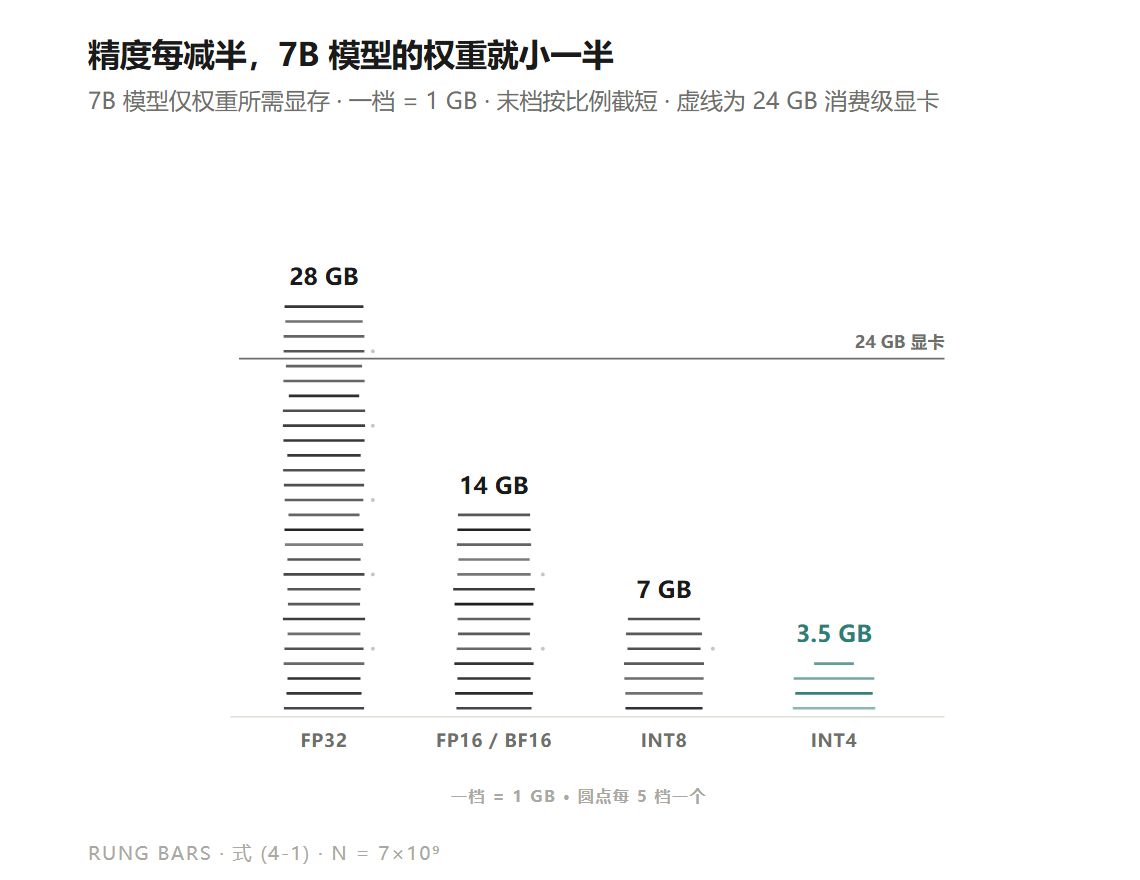
\includegraphics[width=0.49\linewidth]{samples/lf-a.png}\hfill
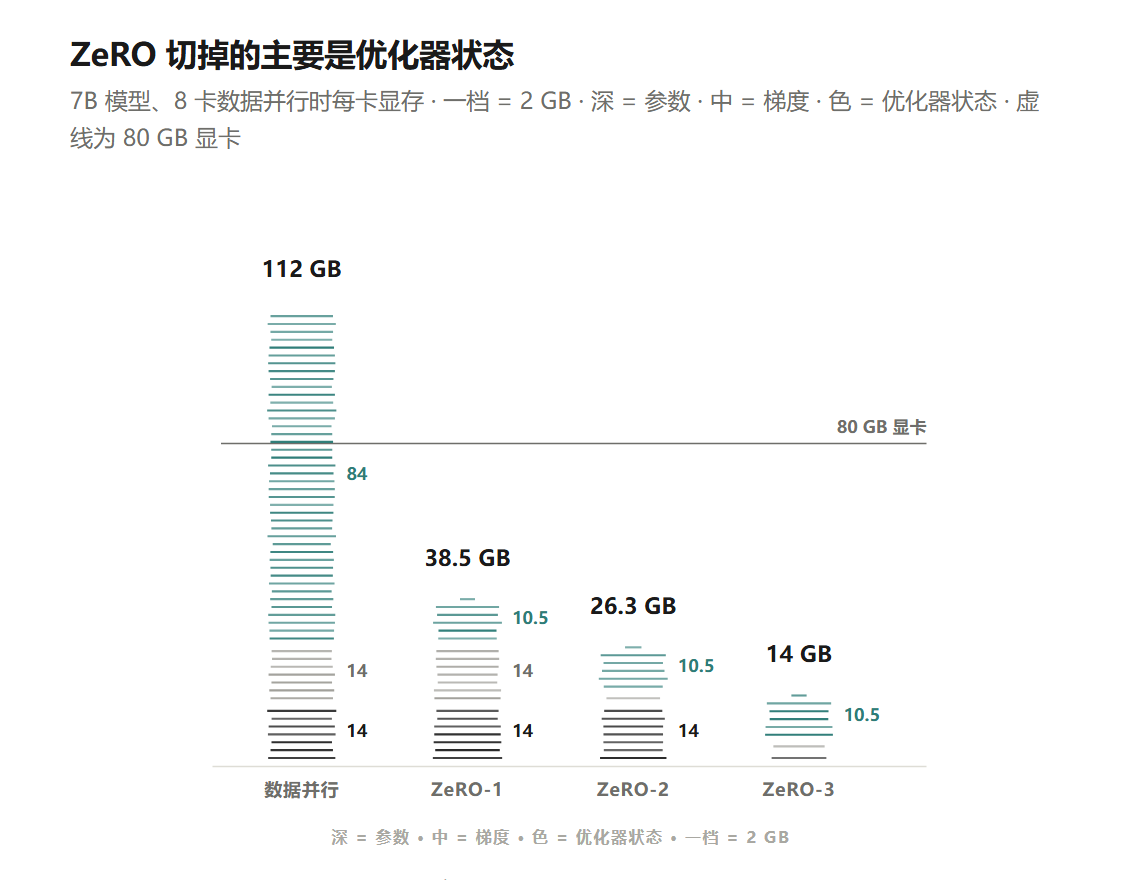
\includegraphics[width=0.49\linewidth]{samples/lf-b.png}
\caption{（样图）左：不同精度下 7B 模型的权重大小；右：ZeRO 各阶段的每卡显存（对应现稿图 4-8）}
\end{figure}

\begin{figure}[H]\centering
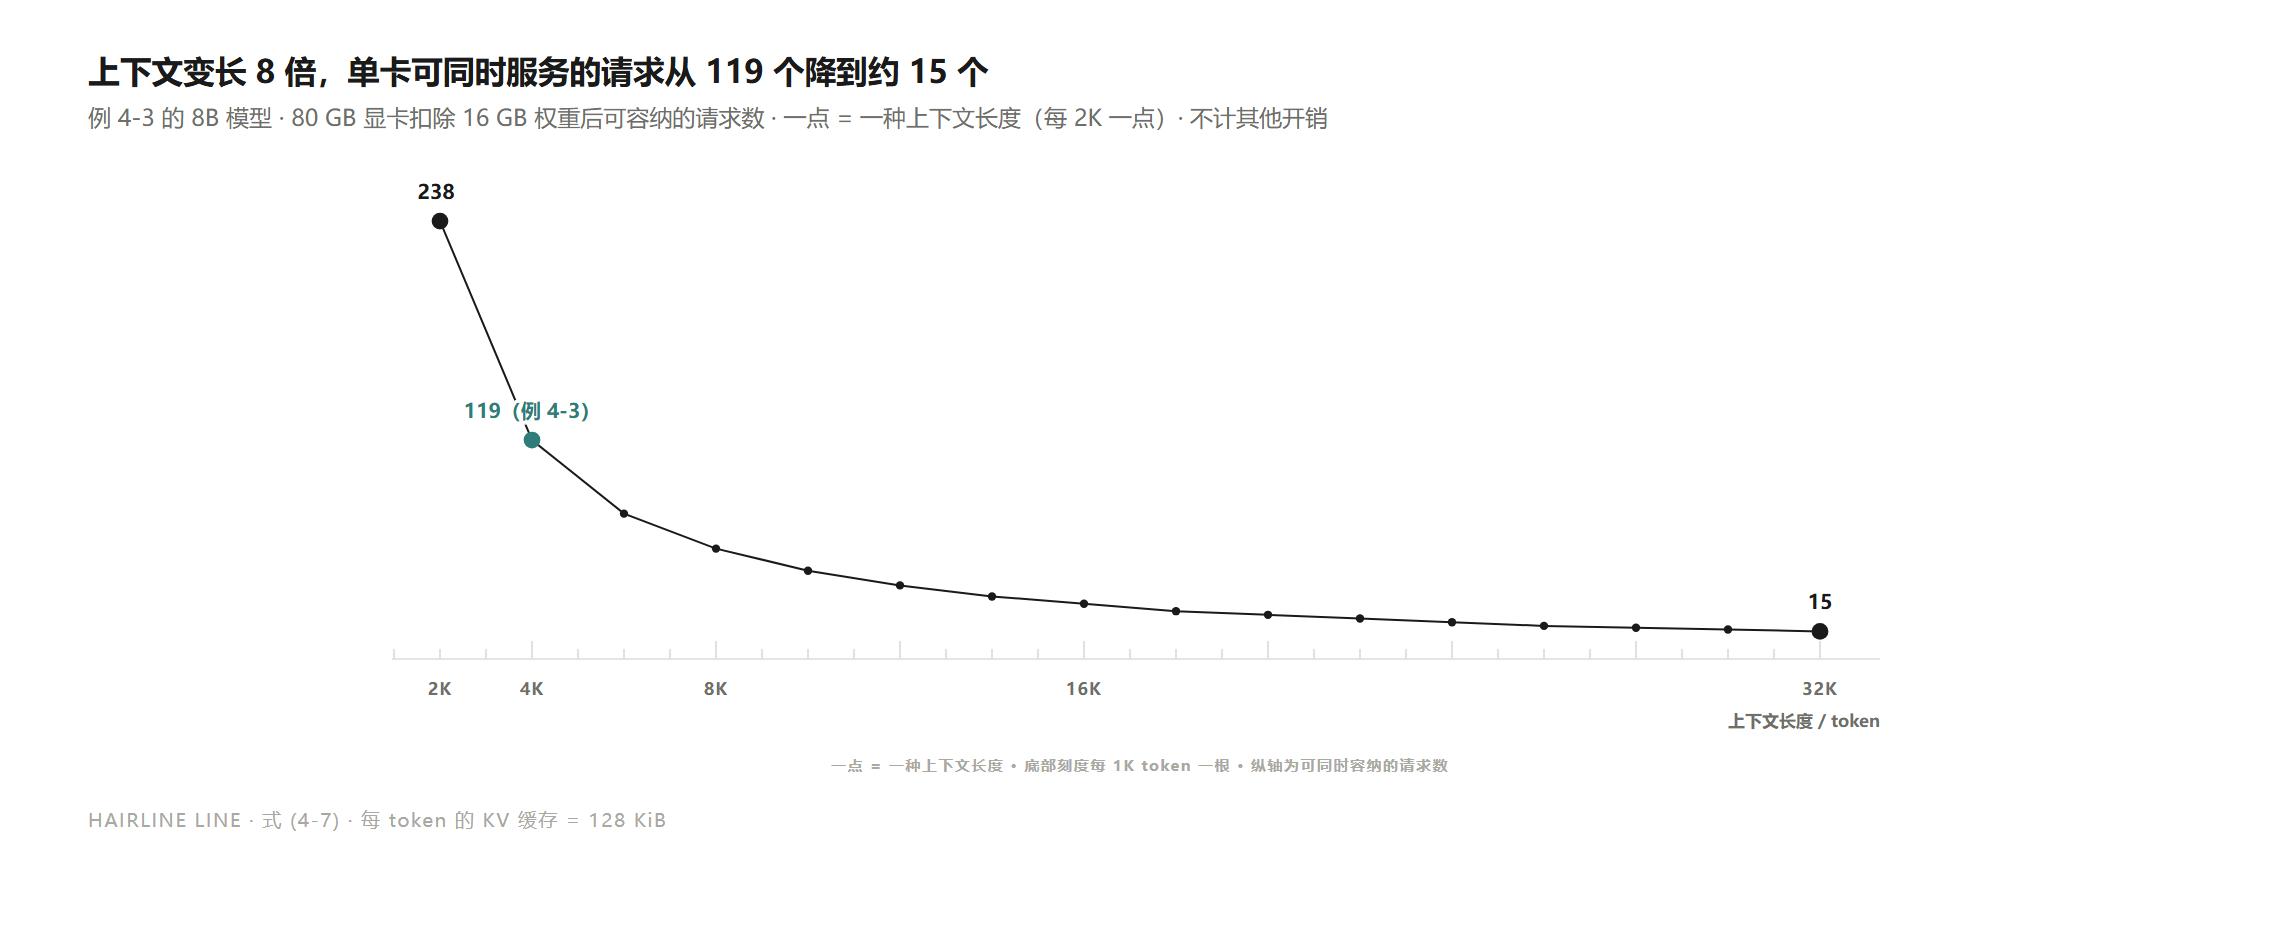
\includegraphics[width=\linewidth]{samples/lf-c.png}
\caption{（样图）上下文长度与单卡可容纳请求数（对应例 4-3）}
\end{figure}

\Needspace{70mm}\noindent\textbf{对照：现稿中用 TikZ / pgfplots 画的同一组数据（图 4-8）}
\begin{figure}[htbp]
\centering
\begin{tikzpicture}[fig]
\begin{axis}[
  xbar stacked, bar width=4.5mm,
  width=0.82\linewidth, height=5.0cm,
  xmin=0, xmax=125, ymin=0.4, ymax=4.6,
  xlabel={每张 GPU 上的模型状态显存 / GB},
  label style={font=\figfont\small}, tick label style={font=\figfont\small},
  ytick={1,2,3,4}, yticklabels={ZeRO-3,ZeRO-2,ZeRO-1,数据并行},
  axis line style={figline}, tick style={figline},
  legend style={font=\figfont\footnotesize, draw=none, at={(0.5,1.03)}, anchor=south, legend columns=3, /tikz/every even column/.append style={column sep=8pt}},
  legend cell align=left,
  clip=false,
]
  \addplot[fill=figline, draw=figline] coordinates {(14,4) (14,3) (14,2) (1.75,1)};
  \addplot[fill=rulegray!45, draw=figline] coordinates {(14,4) (14,3) (1.75,2) (1.75,1)};
  \addplot[fill=accentpale, draw=accent] coordinates {(84,4) (10.5,3) (10.5,2) (10.5,1)};
  \legend{参数（BF16）, 梯度（BF16）, 优化器状态与主权重（FP32）}
  \draw[warn, dashed, line width=0.8pt] (axis cs:80,0.4) -- (axis cs:80,4.6);
  \node[note, text=warn, anchor=south west, font=\figfont\scriptsize] at (axis cs:81,0.45) {单卡 80 GB};
  \node[note, anchor=west] at (axis cs:113,4) {112};
  \node[note, anchor=west] at (axis cs:39.5,3) {38.5};
  \node[note, anchor=west] at (axis cs:27.3,2) {26.3};
  \node[note, anchor=west] at (axis cs:15,1) {14};
\end{axis}
\end{tikzpicture}
\caption{7B 模型在 8 张 GPU 上采用不同 ZeRO 阶段时，每张卡的模型状态显存（BF16 混合精度 + Adam，未计激活值与通信缓冲区）}
\label{fig:zero}
\end{figure}


\end{document}
